\documentclass[1p]{elsarticle_modified}
%\bibliographystyle{elsarticle-num}

%\usepackage[colorlinks]{hyperref}
%\usepackage{abbrmath_seonhwa} %\Abb, \Ascr, \Acal ,\Abf, \Afrak
\usepackage{amsfonts}
\usepackage{amssymb}
\usepackage{amsmath}
\usepackage{amsthm}
\usepackage{scalefnt}
\usepackage{amsbsy}
\usepackage{kotex}
\usepackage{caption}
\usepackage{subfig}
\usepackage{color}
\usepackage{graphicx}
\usepackage{xcolor} %% white, black, red, green, blue, cyan, magenta, yellow
\usepackage{float}
\usepackage{setspace}
\usepackage{hyperref}

\usepackage{tikz}
\usetikzlibrary{arrows}

\usepackage{multirow}
\usepackage{array} % fixed length table
\usepackage{hhline}

%%%%%%%%%%%%%%%%%%%%%
\makeatletter
\renewcommand*\env@matrix[1][\arraystretch]{%
	\edef\arraystretch{#1}%
	\hskip -\arraycolsep
	\let\@ifnextchar\new@ifnextchar
	\array{*\c@MaxMatrixCols c}}
\makeatother %https://tex.stackexchange.com/questions/14071/how-can-i-increase-the-line-spacing-in-a-matrix
%%%%%%%%%%%%%%%

\usepackage[normalem]{ulem}

\newcommand{\msout}[1]{\ifmmode\text{\sout{\ensuremath{#1}}}\else\sout{#1}\fi}
%SOURCE: \msout is \stkout macro in https://tex.stackexchange.com/questions/20609/strikeout-in-math-mode

\newcommand{\cancel}[1]{
	\ifmmode
	{\color{red}\msout{#1}}
	\else
	{\color{red}\sout{#1}}
	\fi
}

\newcommand{\add}[1]{
	{\color{blue}\uwave{#1}}
}

\newcommand{\replace}[2]{
	\ifmmode
	{\color{red}\msout{#1}}{\color{blue}\uwave{#2}}
	\else
	{\color{red}\sout{#1}}{\color{blue}\uwave{#2}}
	\fi
}

\newcommand{\Sol}{\mathcal{S}} %segment
\newcommand{\D}{D} %diagram
\newcommand{\A}{\mathcal{A}} %arc


%%%%%%%%%%%%%%%%%%%%%%%%%%%%%5 test

\def\sl{\operatorname{\textup{SL}}(2,\Cbb)}
\def\psl{\operatorname{\textup{PSL}}(2,\Cbb)}
\def\quan{\mkern 1mu \triangleright \mkern 1mu}

\theoremstyle{definition}
\newtheorem{thm}{Theorem}[section]
\newtheorem{prop}[thm]{Proposition}
\newtheorem{lem}[thm]{Lemma}
\newtheorem{ques}[thm]{Question}
\newtheorem{cor}[thm]{Corollary}
\newtheorem{defn}[thm]{Definition}
\newtheorem{exam}[thm]{Example}
\newtheorem{rmk}[thm]{Remark}
\newtheorem{alg}[thm]{Algorithm}

\newcommand{\I}{\sqrt{-1}}
\begin{document}

%\begin{frontmatter}
%
%\title{Boundary parabolic representations of knots up to 8 crossings}
%
%%% Group authors per affiliation:
%\author{Yunhi Cho} 
%\address{Department of Mathematics, University of Seoul, Seoul, Korea}
%\ead{yhcho@uos.ac.kr}
%
%
%\author{Seonhwa Kim} %\fnref{s_kim}}
%\address{Center for Geometry and Physics, Institute for Basic Science, Pohang, 37673, Korea}
%\ead{ryeona17@ibs.re.kr}
%
%\author{Hyuk Kim}
%\address{Department of Mathematical Sciences, Seoul National University, Seoul 08826, Korea}
%\ead{hyukkim@snu.ac.kr}
%
%\author{Seokbeom Yoon}
%\address{Department of Mathematical Sciences, Seoul National University, Seoul, 08826,  Korea}
%\ead{sbyoon15@snu.ac.kr}
%
%\begin{abstract}
%We find all boundary parabolic representation of knots up to 8 crossings.
%
%\end{abstract}
%\begin{keyword}
%    \MSC[2010] 57M25 
%\end{keyword}
%
%\end{frontmatter}

%\linenumbers
%\tableofcontents
%
\newcommand\colored[1]{\textcolor{white}{\rule[-0.35ex]{0.8em}{1.4ex}}\kern-0.8em\color{red} #1}%
%\newcommand\colored[1]{\textcolor{white}{ #1}\kern-2.17ex	\textcolor{white}{ #1}\kern-1.81ex	\textcolor{white}{ #1}\kern-2.15ex\color{red}#1	}

{\Large $\underline{12n_{0049}~(K12n_{0049})}$}

\setlength{\tabcolsep}{10pt}
\renewcommand{\arraystretch}{1.6}
\vspace{1cm}\begin{tabular}{m{100pt}>{\centering\arraybackslash}m{274pt}}
\multirow{5}{120pt}{
	\centering
	\includegraphics[width=112pt]{../../../GIT/diagram.site/Diagrams/png/2138_12n_0049.png}\\
\ \ \ A knot diagram\footnotemark}&
\allowdisplaybreaks
\textbf{Linearized knot diagam} \\
\cline{2-2}
 &
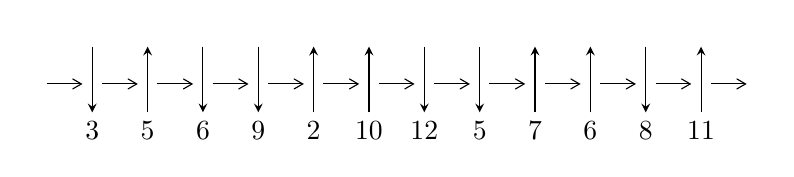
\begin{tikzpicture}[x=20pt, y=17pt]
	% nodes
	\node (C0) at (0, 0) {};
	\node (C1) at (1, 0) {};
	\node (C1U) at (1, +1) {};
	\node (C1D) at (1, -1) {3};

	\node (C2) at (2, 0) {};
	\node (C2U) at (2, +1) {};
	\node (C2D) at (2, -1) {5};

	\node (C3) at (3, 0) {};
	\node (C3U) at (3, +1) {};
	\node (C3D) at (3, -1) {6};

	\node (C4) at (4, 0) {};
	\node (C4U) at (4, +1) {};
	\node (C4D) at (4, -1) {9};

	\node (C5) at (5, 0) {};
	\node (C5U) at (5, +1) {};
	\node (C5D) at (5, -1) {2};

	\node (C6) at (6, 0) {};
	\node (C6U) at (6, +1) {};
	\node (C6D) at (6, -1) {10};

	\node (C7) at (7, 0) {};
	\node (C7U) at (7, +1) {};
	\node (C7D) at (7, -1) {12};

	\node (C8) at (8, 0) {};
	\node (C8U) at (8, +1) {};
	\node (C8D) at (8, -1) {5};

	\node (C9) at (9, 0) {};
	\node (C9U) at (9, +1) {};
	\node (C9D) at (9, -1) {7};

	\node (C10) at (10, 0) {};
	\node (C10U) at (10, +1) {};
	\node (C10D) at (10, -1) {6};

	\node (C11) at (11, 0) {};
	\node (C11U) at (11, +1) {};
	\node (C11D) at (11, -1) {8};

	\node (C12) at (12, 0) {};
	\node (C12U) at (12, +1) {};
	\node (C12D) at (12, -1) {11};
	\node (C13) at (13, 0) {};

	% arrows
	\draw[->,>={angle 60}]
	(C0) edge (C1) (C1) edge (C2) (C2) edge (C3) (C3) edge (C4) (C4) edge (C5) (C5) edge (C6) (C6) edge (C7) (C7) edge (C8) (C8) edge (C9) (C9) edge (C10) (C10) edge (C11) (C11) edge (C12) (C12) edge (C13) ;	\draw[->,>=stealth]
	(C1U) edge (C1D) (C2D) edge (C2U) (C3U) edge (C3D) (C4U) edge (C4D) (C5D) edge (C5U) (C6D) edge (C6U) (C7U) edge (C7D) (C8U) edge (C8D) (C9D) edge (C9U) (C10D) edge (C10U) (C11U) edge (C11D) (C12D) edge (C12U) ;
	\end{tikzpicture} \\
\hhline{~~} \\& 
\textbf{Solving Sequence} \\ \cline{2-2} 
 &
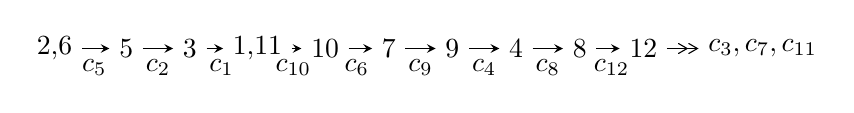
\begin{tikzpicture}[x=23pt, y=7pt]
	% node
	\node (A0) at (-1/8, 0) {2,6};
	\node (A1) at (1, 0) {5};
	\node (A2) at (2, 0) {3};
	\node (A3) at (49/16, 0) {1,11};
	\node (A4) at (33/8, 0) {10};
	\node (A5) at (41/8, 0) {7};
	\node (A6) at (49/8, 0) {9};
	\node (A7) at (57/8, 0) {4};
	\node (A8) at (65/8, 0) {8};
	\node (A9) at (73/8, 0) {12};
	\node (C1) at (1/2, -1) {$c_{5}$};
	\node (C2) at (3/2, -1) {$c_{2}$};
	\node (C3) at (5/2, -1) {$c_{1}$};
	\node (C4) at (29/8, -1) {$c_{10}$};
	\node (C5) at (37/8, -1) {$c_{6}$};
	\node (C6) at (45/8, -1) {$c_{9}$};
	\node (C7) at (53/8, -1) {$c_{4}$};
	\node (C8) at (61/8, -1) {$c_{8}$};
	\node (C9) at (69/8, -1) {$c_{12}$};
	\node (A10) at (11, 0) {$c_{3},c_{7},c_{11}$};

	% edge
	\draw[->,>=stealth]	
	(A0) edge (A1) (A1) edge (A2) (A2) edge (A3) (A3) edge (A4) (A4) edge (A5) (A5) edge (A6) (A6) edge (A7) (A7) edge (A8) (A8) edge (A9) ;
	\draw[->>,>={angle 60}]	
	(A9) edge (A10);
\end{tikzpicture} \\ 

\end{tabular} \\

\footnotetext{
The image of knot diagram is generated by the software ``\textbf{Draw programme}" developed by Andrew Bartholomew(\url{http://www.layer8.co.uk/maths/draw/index.htm\#Running-draw}), where we modified some parts for our purpose(\url{https://github.com/CATsTAILs/LinksPainter}).
}\phantom \\ \newline 
\centering \textbf{Ideals for irreducible components\footnotemark of $X_{\text{par}}$} 
 
\begin{align*}
I^u_{1}&=\langle 
-484296105 u^{35}-876453979 u^{34}+\cdots+5825897536 b+2936630968,\\
\phantom{I^u_{1}}&\phantom{= \langle  }2622553061 u^{35}+6852014457 u^{34}+\cdots+11651795072 a+6583505056,\;u^{36}+2 u^{35}+\cdots-3 u+4\rangle \\
I^u_{2}&=\langle 
-6 a^3 u+44 a^3-29 a^2 u+50 a^2-44 a u+61 b-23 a+26 u-28,\\
\phantom{I^u_{2}}&\phantom{= \langle  }2 a^4-2 a^3 u+5 a^3-2 a^2 u+4 a u-6 a+5 u-3,\;u^2- u+1\rangle \\
I^u_{3}&=\langle 
26 u^3 a^2+8 a^2 u^2-12 u^3 a+15 a^2 u-31 u^2 a-12 u^3+6 a^2+4 a u+40 u^2+71 b-41 a+4 u+30,\\
\phantom{I^u_{3}}&\phantom{= \langle  }2 u^3 a^2+4 a^2 u^2-2 u^3 a+a^3+4 a^2 u-5 u^2 a- u^3-7 a u- u^2-5 a+u+2,\;u^4+u^3+u^2+1\rangle \\
\\
\end{align*}
\raggedright * 3 irreducible components of $\dim_{\mathbb{C}}=0$, with total 56 representations.\\
\footnotetext{All coefficients of polynomials are rational numbers. But the coefficients are sometimes approximated in decimal forms when there is not enough margin.}
\newpage
\renewcommand{\arraystretch}{1}
\centering \section*{I. $I^u_{1}= \langle -4.84\times10^{8} u^{35}-8.76\times10^{8} u^{34}+\cdots+5.83\times10^{9} b+2.94\times10^{9},\;2.62\times10^{9} u^{35}+6.85\times10^{9} u^{34}+\cdots+1.17\times10^{10} a+6.58\times10^{9},\;u^{36}+2 u^{35}+\cdots-3 u+4 \rangle$}
\flushleft \textbf{(i) Arc colorings}\\
\begin{tabular}{m{7pt} m{180pt} m{7pt} m{180pt} }
\flushright $a_{2}=$&$\begin{pmatrix}0\\u\end{pmatrix}$ \\
\flushright $a_{6}=$&$\begin{pmatrix}1\\0\end{pmatrix}$ \\
\flushright $a_{5}=$&$\begin{pmatrix}1\\u^2\end{pmatrix}$ \\
\flushright $a_{3}=$&$\begin{pmatrix}u\\u^3+u\end{pmatrix}$ \\
\flushright $a_{1}=$&$\begin{pmatrix}u^3\\u^5+u^3+u\end{pmatrix}$ \\
\flushright $a_{11}=$&$\begin{pmatrix}-0.225077 u^{35}-0.588065 u^{34}+\cdots-2.43489 u-0.565021\\0.0831282 u^{35}+0.150441 u^{34}+\cdots-0.808963 u-0.504065\end{pmatrix}$ \\
\flushright $a_{10}=$&$\begin{pmatrix}-0.308205 u^{35}-0.738506 u^{34}+\cdots-1.62593 u-0.0609557\\0.0831282 u^{35}+0.150441 u^{34}+\cdots-0.808963 u-0.504065\end{pmatrix}$ \\
\flushright $a_{7}=$&$\begin{pmatrix}0.00526049 u^{35}+0.0984092 u^{34}+\cdots-1.00467 u+1.90403\\-0.130367 u^{35}-0.265551 u^{34}+\cdots+0.257479 u-0.749489\end{pmatrix}$ \\
\flushright $a_{9}=$&$\begin{pmatrix}-0.315652 u^{35}-0.320533 u^{34}+\cdots-3.86030 u+1.93751\\-0.213900 u^{35}-0.524671 u^{34}+\cdots+1.76935 u-2.11821\end{pmatrix}$ \\
\flushright $a_{4}=$&$\begin{pmatrix}- u^3\\u^3+u\end{pmatrix}$ \\
\flushright $a_{8}=$&$\begin{pmatrix}-0.448719 u^{35}-0.603542 u^{34}+\cdots-4.28587 u+1.06239\\-0.174790 u^{35}-0.478417 u^{34}+\cdots+2.25099 u-2.05071\end{pmatrix}$ \\
\flushright $a_{12}=$&$\begin{pmatrix}0.0695792 u^{35}+0.105837 u^{34}+\cdots-0.289164 u+0.533612\\0.106950 u^{35}+0.199836 u^{34}+\cdots+0.0528230 u+0.809104\end{pmatrix}$\\&\end{tabular}
\flushleft \textbf{(ii) Obstruction class $= -1$}\\~\\
\flushleft \textbf{(iii) Cusp Shapes $= \frac{1359975379}{2912948768} u^{35}+\frac{808893889}{1456474384} u^{34}+\cdots+\frac{371799183}{2912948768} u-\frac{4242546469}{728237192}$}\\~\\
\newpage\renewcommand{\arraystretch}{1}
\flushleft \textbf{(iv) u-Polynomials at the component}\newline \\
\begin{tabular}{m{50pt}|m{274pt}}
Crossings & \hspace{64pt}u-Polynomials at each crossing \\
\hline $$\begin{aligned}c_{1}\end{aligned}$$&$\begin{aligned}
&u^{36}+10 u^{35}+\cdots+255 u+16
\end{aligned}$\\
\hline $$\begin{aligned}c_{2},c_{5}\end{aligned}$$&$\begin{aligned}
&u^{36}+2 u^{35}+\cdots-3 u+4
\end{aligned}$\\
\hline $$\begin{aligned}c_{3}\end{aligned}$$&$\begin{aligned}
&u^{36}-2 u^{35}+\cdots+110445 u+62564
\end{aligned}$\\
\hline $$\begin{aligned}c_{4},c_{8}\end{aligned}$$&$\begin{aligned}
&u^{36}-2 u^{35}+\cdots-3584 u+2048
\end{aligned}$\\
\hline $$\begin{aligned}c_{6},c_{9},c_{10}\end{aligned}$$&$\begin{aligned}
&u^{36}+3 u^{35}+\cdots+4 u+1
\end{aligned}$\\
\hline $$\begin{aligned}c_{7},c_{11}\end{aligned}$$&$\begin{aligned}
&u^{36}+3 u^{35}+\cdots+2 u+1
\end{aligned}$\\
\hline $$\begin{aligned}c_{12}\end{aligned}$$&$\begin{aligned}
&u^{36}-23 u^{35}+\cdots-6 u+1
\end{aligned}$\\
\hline
\end{tabular}\\~\\
\newpage\renewcommand{\arraystretch}{1}
\flushleft \textbf{(v) Riley Polynomials at the component}\newline \\
\begin{tabular}{m{50pt}|m{274pt}}
Crossings & \hspace{64pt}Riley Polynomials at each crossing \\
\hline $$\begin{aligned}c_{1}\end{aligned}$$&$\begin{aligned}
&y^{36}+34 y^{35}+\cdots+19807 y+256
\end{aligned}$\\
\hline $$\begin{aligned}c_{2},c_{5}\end{aligned}$$&$\begin{aligned}
&y^{36}+10 y^{35}+\cdots+255 y+16
\end{aligned}$\\
\hline $$\begin{aligned}c_{3}\end{aligned}$$&$\begin{aligned}
&y^{36}+58 y^{35}+\cdots+87628895247 y+3914254096
\end{aligned}$\\
\hline $$\begin{aligned}c_{4},c_{8}\end{aligned}$$&$\begin{aligned}
&y^{36}+30 y^{35}+\cdots+13893632 y+4194304
\end{aligned}$\\
\hline $$\begin{aligned}c_{6},c_{9},c_{10}\end{aligned}$$&$\begin{aligned}
&y^{36}+27 y^{35}+\cdots+6 y+1
\end{aligned}$\\
\hline $$\begin{aligned}c_{7},c_{11}\end{aligned}$$&$\begin{aligned}
&y^{36}+23 y^{35}+\cdots+6 y+1
\end{aligned}$\\
\hline $$\begin{aligned}c_{12}\end{aligned}$$&$\begin{aligned}
&y^{36}-17 y^{35}+\cdots+6 y+1
\end{aligned}$\\
\hline
\end{tabular}\\~\\
\newpage\flushleft \textbf{(vi) Complex Volumes and Cusp Shapes}
$$\begin{array}{c|c|c}  
\text{Solutions to }I^u_{1}& \I (\text{vol} + \sqrt{-1}CS) & \text{Cusp shape}\\
 \hline 
\begin{aligned}
u &= \phantom{-}0.171600 + 1.110920 I \\
a &= -0.204619 + 1.345050 I \\
b &= -0.216810 - 1.196860 I\end{aligned}
 & -4.27639 + 3.16772 I & -7.58797 - 3.35954 I \\ \hline\begin{aligned}
u &= \phantom{-}0.171600 - 1.110920 I \\
a &= -0.204619 - 1.345050 I \\
b &= -0.216810 + 1.196860 I\end{aligned}
 & -4.27639 - 3.16772 I & -7.58797 + 3.35954 I \\ \hline\begin{aligned}
u &= \phantom{-}1.085660 + 0.293972 I \\
a &= \phantom{-}0.392792 - 0.045820 I \\
b &= \phantom{-}0.334592 + 0.680226 I\end{aligned}
 & \phantom{-}4.30159 + 1.64830 I & \phantom{-}7.39222 - 3.81709 I \\ \hline\begin{aligned}
u &= \phantom{-}1.085660 - 0.293972 I \\
a &= \phantom{-}0.392792 + 0.045820 I \\
b &= \phantom{-}0.334592 - 0.680226 I\end{aligned}
 & \phantom{-}4.30159 - 1.64830 I & \phantom{-}7.39222 + 3.81709 I \\ \hline\begin{aligned}
u &= -0.312081 + 0.807793 I \\
a &= \phantom{-}1.53056 + 0.47632 I \\
b &= -0.04471 - 1.51818 I\end{aligned}
 & -7.22153 + 1.57633 I & -9.02842 - 6.04950 I \\ \hline\begin{aligned}
u &= -0.312081 - 0.807793 I \\
a &= \phantom{-}1.53056 - 0.47632 I \\
b &= -0.04471 + 1.51818 I\end{aligned}
 & -7.22153 - 1.57633 I & -9.02842 + 6.04950 I \\ \hline\begin{aligned}
u &= \phantom{-}0.633550 + 0.959306 I \\
a &= \phantom{-}1.67177 + 0.11512 I \\
b &= \phantom{-}0.190966 + 0.946097 I\end{aligned}
 & -1.10855 + 3.29892 I & -6.24385 - 2.89898 I \\ \hline\begin{aligned}
u &= \phantom{-}0.633550 - 0.959306 I \\
a &= \phantom{-}1.67177 - 0.11512 I \\
b &= \phantom{-}0.190966 - 0.946097 I\end{aligned}
 & -1.10855 - 3.29892 I & -6.24385 + 2.89898 I \\ \hline\begin{aligned}
u &= \phantom{-}0.923008 + 0.689836 I \\
a &= -0.417168 - 0.169238 I \\
b &= -0.346298 + 0.404592 I\end{aligned}
 & \phantom{-}3.90051 + 1.86347 I & \phantom{-}6.48131 - 1.21859 I \\ \hline\begin{aligned}
u &= \phantom{-}0.923008 - 0.689836 I \\
a &= -0.417168 + 0.169238 I \\
b &= -0.346298 - 0.404592 I\end{aligned}
 & \phantom{-}3.90051 - 1.86347 I & \phantom{-}6.48131 + 1.21859 I\\
 \hline 
 \end{array}$$\newpage$$\begin{array}{c|c|c}  
\text{Solutions to }I^u_{1}& \I (\text{vol} + \sqrt{-1}CS) & \text{Cusp shape}\\
 \hline 
\begin{aligned}
u &= -0.874677 + 0.761101 I \\
a &= -0.370685 - 0.647821 I \\
b &= -0.59935 - 1.30228 I\end{aligned}
 & \phantom{-}3.00591 + 2.79905 I & -0.254837 - 1.357172 I \\ \hline\begin{aligned}
u &= -0.874677 - 0.761101 I \\
a &= -0.370685 + 0.647821 I \\
b &= -0.59935 + 1.30228 I\end{aligned}
 & \phantom{-}3.00591 - 2.79905 I & -0.254837 + 1.357172 I \\ \hline\begin{aligned}
u &= -0.433561 + 0.706966 I \\
a &= -1.95347 - 0.21519 I \\
b &= -0.16134 + 1.55299 I\end{aligned}
 & -6.76494 - 4.64397 I & -3.32082 - 3.17287 I \\ \hline\begin{aligned}
u &= -0.433561 - 0.706966 I \\
a &= -1.95347 + 0.21519 I \\
b &= -0.16134 - 1.55299 I\end{aligned}
 & -6.76494 + 4.64397 I & -3.32082 + 3.17287 I \\ \hline\begin{aligned}
u &= \phantom{-}0.458151 + 0.676958 I \\
a &= \phantom{-}0.753522 - 0.718675 I \\
b &= \phantom{-}0.019557 - 0.666846 I\end{aligned}
 & -0.198612 + 1.374800 I & -3.09098 - 4.69147 I \\ \hline\begin{aligned}
u &= \phantom{-}0.458151 - 0.676958 I \\
a &= \phantom{-}0.753522 + 0.718675 I \\
b &= \phantom{-}0.019557 + 0.666846 I\end{aligned}
 & -0.198612 - 1.374800 I & -3.09098 + 4.69147 I \\ \hline\begin{aligned}
u &= \phantom{-}0.471893 + 1.096490 I \\
a &= \phantom{-}0.224206 + 0.323614 I \\
b &= \phantom{-}0.422956 - 0.007097 I\end{aligned}
 & \phantom{-}1.60525 + 3.66384 I & \phantom{-}4.88856 - 3.83188 I \\ \hline\begin{aligned}
u &= \phantom{-}0.471893 - 1.096490 I \\
a &= \phantom{-}0.224206 - 0.323614 I \\
b &= \phantom{-}0.422956 + 0.007097 I\end{aligned}
 & \phantom{-}1.60525 - 3.66384 I & \phantom{-}4.88856 + 3.83188 I \\ \hline\begin{aligned}
u &= -1.024050 + 0.695309 I \\
a &= \phantom{-}0.535986 + 0.556491 I \\
b &= \phantom{-}0.567012 + 1.295000 I\end{aligned}
 & \phantom{-}7.75189 + 8.17134 I & \phantom{-}1.99685 - 4.00929 I \\ \hline\begin{aligned}
u &= -1.024050 - 0.695309 I \\
a &= \phantom{-}0.535986 - 0.556491 I \\
b &= \phantom{-}0.567012 - 1.295000 I\end{aligned}
 & \phantom{-}7.75189 - 8.17134 I & \phantom{-}1.99685 + 4.00929 I\\
 \hline 
 \end{array}$$\newpage$$\begin{array}{c|c|c}  
\text{Solutions to }I^u_{1}& \I (\text{vol} + \sqrt{-1}CS) & \text{Cusp shape}\\
 \hline 
\begin{aligned}
u &= -0.961809 + 0.820602 I \\
a &= \phantom{-}1.181150 + 0.495596 I \\
b &= \phantom{-}1.059240 - 0.084079 I\end{aligned}
 & \phantom{-}11.48810 + 2.42769 I & \phantom{-}4.62667 - 0.56621 I \\ \hline\begin{aligned}
u &= -0.961809 - 0.820602 I \\
a &= \phantom{-}1.181150 - 0.495596 I \\
b &= \phantom{-}1.059240 + 0.084079 I\end{aligned}
 & \phantom{-}11.48810 - 2.42769 I & \phantom{-}4.62667 + 0.56621 I \\ \hline\begin{aligned}
u &= -0.785168 + 1.017390 I \\
a &= -1.76172 - 0.30795 I \\
b &= -0.54057 + 1.40007 I\end{aligned}
 & \phantom{-}2.20898 - 8.97826 I & -1.63229 + 5.82526 I \\ \hline\begin{aligned}
u &= -0.785168 - 1.017390 I \\
a &= -1.76172 + 0.30795 I \\
b &= -0.54057 - 1.40007 I\end{aligned}
 & \phantom{-}2.20898 + 8.97826 I & -1.63229 - 5.82526 I \\ \hline\begin{aligned}
u &= -0.854722 + 1.028010 I \\
a &= \phantom{-}1.038600 + 0.610663 I \\
b &= \phantom{-}1.088070 - 0.034474 I\end{aligned}
 & \phantom{-}10.81730 - 9.09210 I & \phantom{-}3.56135 + 5.43028 I \\ \hline\begin{aligned}
u &= -0.854722 - 1.028010 I \\
a &= \phantom{-}1.038600 - 0.610663 I \\
b &= \phantom{-}1.088070 + 0.034474 I\end{aligned}
 & \phantom{-}10.81730 + 9.09210 I & \phantom{-}3.56135 - 5.43028 I \\ \hline\begin{aligned}
u &= -0.810811 + 1.108300 I \\
a &= \phantom{-}1.71062 + 0.36230 I \\
b &= \phantom{-}0.53618 - 1.37404 I\end{aligned}
 & \phantom{-}6.4290 - 14.8448 I & \phantom{-}0.25659 + 8.03190 I \\ \hline\begin{aligned}
u &= -0.810811 - 1.108300 I \\
a &= \phantom{-}1.71062 - 0.36230 I \\
b &= \phantom{-}0.53618 + 1.37404 I\end{aligned}
 & \phantom{-}6.4290 + 14.8448 I & \phantom{-}0.25659 - 8.03190 I \\ \hline\begin{aligned}
u &= \phantom{-}0.310580 + 1.362320 I \\
a &= \phantom{-}0.544180 - 0.799588 I \\
b &= \phantom{-}0.307951 + 1.137470 I\end{aligned}
 & -1.47960 + 6.60474 I & -1.77461 - 8.22994 I \\ \hline\begin{aligned}
u &= \phantom{-}0.310580 - 1.362320 I \\
a &= \phantom{-}0.544180 + 0.799588 I \\
b &= \phantom{-}0.307951 - 1.137470 I\end{aligned}
 & -1.47960 - 6.60474 I & -1.77461 + 8.22994 I\\
 \hline 
 \end{array}$$\newpage$$\begin{array}{c|c|c}  
\text{Solutions to }I^u_{1}& \I (\text{vol} + \sqrt{-1}CS) & \text{Cusp shape}\\
 \hline 
\begin{aligned}
u &= \phantom{-}0.92557 + 1.09311 I \\
a &= -0.857998 + 0.114331 I \\
b &= -0.322915 - 0.915206 I\end{aligned}
 & \phantom{-}2.65507 + 4.99154 I & \phantom{-}3.97038 - 7.84261 I \\ \hline\begin{aligned}
u &= \phantom{-}0.92557 - 1.09311 I \\
a &= -0.857998 - 0.114331 I \\
b &= -0.322915 + 0.915206 I\end{aligned}
 & \phantom{-}2.65507 - 4.99154 I & \phantom{-}3.97038 + 7.84261 I \\ \hline\begin{aligned}
u &= -0.165244 + 0.479278 I \\
a &= -1.83465 - 0.61814 I \\
b &= -0.570372 + 0.472484 I\end{aligned}
 & \phantom{-}0.02049 - 1.94674 I & -0.99192 + 2.87831 I \\ \hline\begin{aligned}
u &= -0.165244 - 0.479278 I \\
a &= -1.83465 + 0.61814 I \\
b &= -0.570372 - 0.472484 I\end{aligned}
 & \phantom{-}0.02049 + 1.94674 I & -0.99192 - 2.87831 I \\ \hline\begin{aligned}
u &= \phantom{-}0.242112 + 0.308667 I \\
a &= \phantom{-}0.941920 - 0.135172 I \\
b &= -0.224155 - 0.681318 I\end{aligned}
 & -0.235696 + 1.266250 I & -2.12322 - 5.45165 I \\ \hline\begin{aligned}
u &= \phantom{-}0.242112 - 0.308667 I \\
a &= \phantom{-}0.941920 + 0.135172 I \\
b &= -0.224155 + 0.681318 I\end{aligned}
 & -0.235696 - 1.266250 I & -2.12322 + 5.45165 I\\
 \hline 
 \end{array}$$\newpage\newpage\renewcommand{\arraystretch}{1}
\centering \section*{II. $I^u_{2}= \langle -6 a^3 u-29 a^2 u+\cdots-23 a-28,\;-2 a^3 u-2 a^2 u+\cdots-6 a-3,\;u^2- u+1 \rangle$}
\flushleft \textbf{(i) Arc colorings}\\
\begin{tabular}{m{7pt} m{180pt} m{7pt} m{180pt} }
\flushright $a_{2}=$&$\begin{pmatrix}0\\u\end{pmatrix}$ \\
\flushright $a_{6}=$&$\begin{pmatrix}1\\0\end{pmatrix}$ \\
\flushright $a_{5}=$&$\begin{pmatrix}1\\u-1\end{pmatrix}$ \\
\flushright $a_{3}=$&$\begin{pmatrix}u\\u-1\end{pmatrix}$ \\
\flushright $a_{1}=$&$\begin{pmatrix}-1\\0\end{pmatrix}$ \\
\flushright $a_{11}=$&$\begin{pmatrix}a\\0.0983607 a^{3} u+0.475410 a^{2} u+\cdots+0.377049 a+0.459016\end{pmatrix}$ \\
\flushright $a_{10}=$&$\begin{pmatrix}-0.0983607 a^{3} u-0.475410 a^{2} u+\cdots+0.622951 a-0.459016\\0.0983607 a^{3} u+0.475410 a^{2} u+\cdots+0.377049 a+0.459016\end{pmatrix}$ \\
\flushright $a_{7}=$&$\begin{pmatrix}1.18033 a^{3} u-0.295082 a^{2} u+\cdots+0.524590 a-0.491803\\-0.786885 a^{3} u+0.196721 a^{2} u+\cdots+0.983607 a+2.32787\end{pmatrix}$ \\
\flushright $a_{9}=$&$\begin{pmatrix}0.196721 a^{3} u+0.950820 a^{2} u+\cdots+0.754098 a+0.918033\\-1.44262 a^{3} u-1.63934 a^{2} u+\cdots-0.196721 a+0.934426\end{pmatrix}$ \\
\flushright $a_{4}=$&$\begin{pmatrix}1\\u-1\end{pmatrix}$ \\
\flushright $a_{8}=$&$\begin{pmatrix}0.196721 a^{3} u+0.950820 a^{2} u+\cdots+0.754098 a+0.918033\\-1.44262 a^{3} u-1.63934 a^{2} u+\cdots-0.196721 a+0.934426\end{pmatrix}$ \\
\flushright $a_{12}=$&$\begin{pmatrix}0.393443 a^{3} u-0.0983607 a^{2} u+\cdots+1.50820 a-0.163934\\-0.786885 a^{3} u+0.196721 a^{2} u+\cdots+0.983607 a+2.32787\end{pmatrix}$\\&\end{tabular}
\flushleft \textbf{(ii) Obstruction class $= 1$}\\~\\
\flushleft \textbf{(iii) Cusp Shapes $= \frac{70}{61} a^3 u-\frac{188}{61} a^3-\frac{48}{61} a^2 u-\frac{136}{61} a^2-\frac{56}{61} a u+\frac{248}{61} a-\frac{344}{61} u+\frac{347}{61}$}\\~\\
\newpage\renewcommand{\arraystretch}{1}
\flushleft \textbf{(iv) u-Polynomials at the component}\newline \\
\begin{tabular}{m{50pt}|m{274pt}}
Crossings & \hspace{64pt}u-Polynomials at each crossing \\
\hline $$\begin{aligned}c_{1},c_{3},c_{5}\end{aligned}$$&$\begin{aligned}
&(u^2- u+1)^4
\end{aligned}$\\
\hline $$\begin{aligned}c_{2}\end{aligned}$$&$\begin{aligned}
&(u^2+u+1)^4
\end{aligned}$\\
\hline $$\begin{aligned}c_{4},c_{8}\end{aligned}$$&$\begin{aligned}
&u^8
\end{aligned}$\\
\hline $$\begin{aligned}c_{6}\end{aligned}$$&$\begin{aligned}
&(u^4+u^3+3 u^2+2 u+1)^2
\end{aligned}$\\
\hline $$\begin{aligned}c_{7}\end{aligned}$$&$\begin{aligned}
&(u^4+u^3+u^2+1)^2
\end{aligned}$\\
\hline $$\begin{aligned}c_{9},c_{10},c_{12}\end{aligned}$$&$\begin{aligned}
&(u^4- u^3+3 u^2-2 u+1)^2
\end{aligned}$\\
\hline $$\begin{aligned}c_{11}\end{aligned}$$&$\begin{aligned}
&(u^4- u^3+u^2+1)^2
\end{aligned}$\\
\hline
\end{tabular}\\~\\
\newpage\renewcommand{\arraystretch}{1}
\flushleft \textbf{(v) Riley Polynomials at the component}\newline \\
\begin{tabular}{m{50pt}|m{274pt}}
Crossings & \hspace{64pt}Riley Polynomials at each crossing \\
\hline $$\begin{aligned}c_{1},c_{2},c_{3}\\c_{5}\end{aligned}$$&$\begin{aligned}
&(y^2+y+1)^4
\end{aligned}$\\
\hline $$\begin{aligned}c_{4},c_{8}\end{aligned}$$&$\begin{aligned}
&y^8
\end{aligned}$\\
\hline $$\begin{aligned}c_{6},c_{9},c_{10}\\c_{12}\end{aligned}$$&$\begin{aligned}
&(y^4+5 y^3+7 y^2+2 y+1)^2
\end{aligned}$\\
\hline $$\begin{aligned}c_{7},c_{11}\end{aligned}$$&$\begin{aligned}
&(y^4+y^3+3 y^2+2 y+1)^2
\end{aligned}$\\
\hline
\end{tabular}\\~\\
\newpage\flushleft \textbf{(vi) Complex Volumes and Cusp Shapes}
$$\begin{array}{c|c|c}  
\text{Solutions to }I^u_{2}& \I (\text{vol} + \sqrt{-1}CS) & \text{Cusp shape}\\
 \hline 
\begin{aligned}
u &= \phantom{-}0.500000 + 0.866025 I \\
a &= -0.334772 + 0.902624 I \\
b &= -0.395123 + 0.506844 I\end{aligned}
 & \phantom{-}0.211005 + 0.614778 I & \phantom{-}2.28131 + 2.56093 I \\ \hline\begin{aligned}
u &= \phantom{-}0.500000 + 0.866025 I \\
a &= \phantom{-}1.118210 - 0.202000 I \\
b &= -0.10488 + 1.55249 I\end{aligned}
 & -6.79074 - 1.13408 I & \phantom{-}0.84181 - 3.00733 I \\ \hline\begin{aligned}
u &= \phantom{-}0.500000 + 0.866025 I \\
a &= -1.212650 - 0.218250 I \\
b &= -0.395123 - 0.506844 I\end{aligned}
 & \phantom{-}0.21101 + 3.44499 I & -0.06504 - 6.27596 I \\ \hline\begin{aligned}
u &= \phantom{-}0.500000 + 0.866025 I \\
a &= -1.57079 + 0.38365 I \\
b &= -0.10488 - 1.55249 I\end{aligned}
 & -6.79074 + 5.19385 I & -4.18309 - 10.81465 I \\ \hline\begin{aligned}
u &= \phantom{-}0.500000 - 0.866025 I \\
a &= -0.334772 - 0.902624 I \\
b &= -0.395123 - 0.506844 I\end{aligned}
 & \phantom{-}0.211005 - 0.614778 I & \phantom{-}2.28131 - 2.56093 I \\ \hline\begin{aligned}
u &= \phantom{-}0.500000 - 0.866025 I \\
a &= \phantom{-}1.118210 + 0.202000 I \\
b &= -0.10488 - 1.55249 I\end{aligned}
 & -6.79074 + 1.13408 I & \phantom{-}0.84181 + 3.00733 I \\ \hline\begin{aligned}
u &= \phantom{-}0.500000 - 0.866025 I \\
a &= -1.212650 + 0.218250 I \\
b &= -0.395123 + 0.506844 I\end{aligned}
 & \phantom{-}0.21101 - 3.44499 I & -0.06504 + 6.27596 I \\ \hline\begin{aligned}
u &= \phantom{-}0.500000 - 0.866025 I \\
a &= -1.57079 - 0.38365 I \\
b &= -0.10488 + 1.55249 I\end{aligned}
 & -6.79074 - 5.19385 I & -4.18309 + 10.81465 I\\
 \hline 
 \end{array}$$\newpage\newpage\renewcommand{\arraystretch}{1}
\centering \section*{III. $I^u_{3}= \langle 26 u^3 a^2-12 u^3 a+\cdots-41 a+30,\;2 u^3 a^2-2 u^3 a+\cdots-5 a+2,\;u^4+u^3+u^2+1 \rangle$}
\flushleft \textbf{(i) Arc colorings}\\
\begin{tabular}{m{7pt} m{180pt} m{7pt} m{180pt} }
\flushright $a_{2}=$&$\begin{pmatrix}0\\u\end{pmatrix}$ \\
\flushright $a_{6}=$&$\begin{pmatrix}1\\0\end{pmatrix}$ \\
\flushright $a_{5}=$&$\begin{pmatrix}1\\u^2\end{pmatrix}$ \\
\flushright $a_{3}=$&$\begin{pmatrix}u\\u^3+u\end{pmatrix}$ \\
\flushright $a_{1}=$&$\begin{pmatrix}u^3\\u^3+u^2+1\end{pmatrix}$ \\
\flushright $a_{11}=$&$\begin{pmatrix}a\\-0.366197 a^{2} u^{3}+0.169014 a u^{3}+\cdots+0.577465 a-0.422535\end{pmatrix}$ \\
\flushright $a_{10}=$&$\begin{pmatrix}0.366197 a^{2} u^{3}-0.169014 a u^{3}+\cdots+0.422535 a+0.422535\\-0.366197 a^{2} u^{3}+0.169014 a u^{3}+\cdots+0.577465 a-0.422535\end{pmatrix}$ \\
\flushright $a_{7}=$&$\begin{pmatrix}-0.267606 a^{2} u^{3}+0.661972 a u^{3}+\cdots-1.15493 a+0.845070\\0.239437 a^{2} u^{3}+0.197183 a u^{3}+\cdots+0.507042 a+0.507042\end{pmatrix}$ \\
\flushright $a_{9}=$&$\begin{pmatrix}u^2+1\\- u^3- u^2-1\end{pmatrix}$ \\
\flushright $a_{4}=$&$\begin{pmatrix}- u^3\\u^3+u\end{pmatrix}$ \\
\flushright $a_{8}=$&$\begin{pmatrix}1\\0\end{pmatrix}$ \\
\flushright $a_{12}=$&$\begin{pmatrix}-0.366197 a^{2} u^{3}+0.169014 a u^{3}+\cdots-0.422535 a-0.422535\\0.366197 a^{2} u^{3}-0.169014 a u^{3}+\cdots-0.577465 a+0.422535\end{pmatrix}$\\&\end{tabular}
\flushleft \textbf{(ii) Obstruction class $= -1$}\\~\\
\flushleft \textbf{(iii) Cusp Shapes $= -4 u^2-4 u-2$}\\~\\
\newpage\renewcommand{\arraystretch}{1}
\flushleft \textbf{(iv) u-Polynomials at the component}\newline \\
\begin{tabular}{m{50pt}|m{274pt}}
Crossings & \hspace{64pt}u-Polynomials at each crossing \\
\hline $$\begin{aligned}c_{1},c_{4},c_{8}\end{aligned}$$&$\begin{aligned}
&(u^4+u^3+3 u^2+2 u+1)^3
\end{aligned}$\\
\hline $$\begin{aligned}c_{2},c_{5}\end{aligned}$$&$\begin{aligned}
&(u^4+u^3+u^2+1)^3
\end{aligned}$\\
\hline $$\begin{aligned}c_{3}\end{aligned}$$&$\begin{aligned}
&(u^4- u^3+5 u^2+u+2)^3
\end{aligned}$\\
\hline $$\begin{aligned}c_{6},c_{7},c_{9}\\c_{10},c_{11}\end{aligned}$$&$\begin{aligned}
&u^{12}+4 u^{10}+\cdots-2 u+1
\end{aligned}$\\
\hline $$\begin{aligned}c_{12}\end{aligned}$$&$\begin{aligned}
&u^{12}-8 u^{11}+\cdots-10 u+1
\end{aligned}$\\
\hline
\end{tabular}\\~\\
\newpage\renewcommand{\arraystretch}{1}
\flushleft \textbf{(v) Riley Polynomials at the component}\newline \\
\begin{tabular}{m{50pt}|m{274pt}}
Crossings & \hspace{64pt}Riley Polynomials at each crossing \\
\hline $$\begin{aligned}c_{1},c_{4},c_{8}\end{aligned}$$&$\begin{aligned}
&(y^4+5 y^3+7 y^2+2 y+1)^3
\end{aligned}$\\
\hline $$\begin{aligned}c_{2},c_{5}\end{aligned}$$&$\begin{aligned}
&(y^4+y^3+3 y^2+2 y+1)^3
\end{aligned}$\\
\hline $$\begin{aligned}c_{3}\end{aligned}$$&$\begin{aligned}
&(y^4+9 y^3+31 y^2+19 y+4)^3
\end{aligned}$\\
\hline $$\begin{aligned}c_{6},c_{7},c_{9}\\c_{10},c_{11}\end{aligned}$$&$\begin{aligned}
&y^{12}+8 y^{11}+\cdots+10 y+1
\end{aligned}$\\
\hline $$\begin{aligned}c_{12}\end{aligned}$$&$\begin{aligned}
&y^{12}-8 y^{11}+\cdots+2 y+1
\end{aligned}$\\
\hline
\end{tabular}\\~\\
\newpage\flushleft \textbf{(vi) Complex Volumes and Cusp Shapes}
$$\begin{array}{c|c|c}  
\text{Solutions to }I^u_{3}& \I (\text{vol} + \sqrt{-1}CS) & \text{Cusp shape}\\
 \hline 
\begin{aligned}
u &= \phantom{-}0.351808 + 0.720342 I \\
a &= \phantom{-}0.266204 - 0.424111 I \\
b &= -0.202218 - 0.425275 I\end{aligned}
 & -0.21101 + 1.41510 I & -1.82674 - 4.90874 I \\ \hline\begin{aligned}
u &= \phantom{-}0.351808 + 0.720342 I \\
a &= \phantom{-}1.61961 - 0.46490 I \\
b &= \phantom{-}0.169110 - 0.735861 I\end{aligned}
 & -0.21101 + 1.41510 I & -1.82674 - 4.90874 I \\ \hline\begin{aligned}
u &= \phantom{-}0.351808 + 0.720342 I \\
a &= -0.70433 - 3.80711 I \\
b &= \phantom{-}0.033108 + 1.161140 I\end{aligned}
 & -0.21101 + 1.41510 I & -1.82674 - 4.90874 I \\ \hline\begin{aligned}
u &= \phantom{-}0.351808 - 0.720342 I \\
a &= \phantom{-}0.266204 + 0.424111 I \\
b &= -0.202218 + 0.425275 I\end{aligned}
 & -0.21101 - 1.41510 I & -1.82674 + 4.90874 I \\ \hline\begin{aligned}
u &= \phantom{-}0.351808 - 0.720342 I \\
a &= \phantom{-}1.61961 + 0.46490 I \\
b &= \phantom{-}0.169110 + 0.735861 I\end{aligned}
 & -0.21101 - 1.41510 I & -1.82674 + 4.90874 I \\ \hline\begin{aligned}
u &= \phantom{-}0.351808 - 0.720342 I \\
a &= -0.70433 + 3.80711 I \\
b &= \phantom{-}0.033108 - 1.161140 I\end{aligned}
 & -0.21101 - 1.41510 I & -1.82674 + 4.90874 I \\ \hline\begin{aligned}
u &= -0.851808 + 0.911292 I \\
a &= -1.140580 - 0.606578 I \\
b &= -1.096690 + 0.070743 I\end{aligned}
 & \phantom{-}6.79074 - 3.16396 I & \phantom{-}1.82674 + 2.56480 I \\ \hline\begin{aligned}
u &= -0.851808 + 0.911292 I \\
a &= \phantom{-}0.220330 + 0.512696 I \\
b &= \phantom{-}0.59056 + 1.34306 I\end{aligned}
 & \phantom{-}6.79074 - 3.16396 I & \phantom{-}1.82674 + 2.56480 I \\ \hline\begin{aligned}
u &= -0.851808 + 0.911292 I \\
a &= \phantom{-}1.73877 + 0.20498 I \\
b &= \phantom{-}0.50613 - 1.41380 I\end{aligned}
 & \phantom{-}6.79074 - 3.16396 I & \phantom{-}1.82674 + 2.56480 I \\ \hline\begin{aligned}
u &= -0.851808 - 0.911292 I \\
a &= -1.140580 + 0.606578 I \\
b &= -1.096690 - 0.070743 I\end{aligned}
 & \phantom{-}6.79074 + 3.16396 I & \phantom{-}1.82674 - 2.56480 I\\
 \hline 
 \end{array}$$\newpage$$\begin{array}{c|c|c}  
\text{Solutions to }I^u_{3}& \I (\text{vol} + \sqrt{-1}CS) & \text{Cusp shape}\\
 \hline 
\begin{aligned}
u &= -0.851808 - 0.911292 I \\
a &= \phantom{-}0.220330 - 0.512696 I \\
b &= \phantom{-}0.59056 - 1.34306 I\end{aligned}
 & \phantom{-}6.79074 + 3.16396 I & \phantom{-}1.82674 - 2.56480 I \\ \hline\begin{aligned}
u &= -0.851808 - 0.911292 I \\
a &= \phantom{-}1.73877 - 0.20498 I \\
b &= \phantom{-}0.50613 + 1.41380 I\end{aligned}
 & \phantom{-}6.79074 + 3.16396 I & \phantom{-}1.82674 - 2.56480 I\\
 \hline 
 \end{array}$$\newpage
\newpage\renewcommand{\arraystretch}{1}
\centering \section*{ IV. u-Polynomials}
\begin{tabular}{m{50pt}|m{274pt}}
Crossings & \hspace{64pt}u-Polynomials at each crossing \\
\hline $$\begin{aligned}c_{1}\end{aligned}$$&$\begin{aligned}
&(u^2- u+1)^4(u^4+u^3+3 u^2+2 u+1)^3\\
&\cdot(u^{36}+10 u^{35}+\cdots+255 u+16)
\end{aligned}$\\
\hline $$\begin{aligned}c_{2}\end{aligned}$$&$\begin{aligned}
&((u^2+u+1)^4)(u^4+u^3+u^2+1)^3(u^{36}+2 u^{35}+\cdots-3 u+4)
\end{aligned}$\\
\hline $$\begin{aligned}c_{3}\end{aligned}$$&$\begin{aligned}
&(u^2- u+1)^4(u^4- u^3+5 u^2+u+2)^3\\
&\cdot(u^{36}-2 u^{35}+\cdots+110445 u+62564)
\end{aligned}$\\
\hline $$\begin{aligned}c_{4},c_{8}\end{aligned}$$&$\begin{aligned}
&u^8(u^4+u^3+3 u^2+2 u+1)^{3}(u^{36}-2 u^{35}+\cdots-3584 u+2048)
\end{aligned}$\\
\hline $$\begin{aligned}c_{5}\end{aligned}$$&$\begin{aligned}
&((u^2- u+1)^4)(u^4+u^3+u^2+1)^3(u^{36}+2 u^{35}+\cdots-3 u+4)
\end{aligned}$\\
\hline $$\begin{aligned}c_{6}\end{aligned}$$&$\begin{aligned}
&((u^4+u^3+3 u^2+2 u+1)^2)(u^{12}+4 u^{10}+\cdots-2 u+1)\\
&\cdot(u^{36}+3 u^{35}+\cdots+4 u+1)
\end{aligned}$\\
\hline $$\begin{aligned}c_{7}\end{aligned}$$&$\begin{aligned}
&((u^4+u^3+u^2+1)^2)(u^{12}+4 u^{10}+\cdots-2 u+1)(u^{36}+3 u^{35}+\cdots+2 u+1)
\end{aligned}$\\
\hline $$\begin{aligned}c_{9},c_{10}\end{aligned}$$&$\begin{aligned}
&((u^4- u^3+3 u^2-2 u+1)^2)(u^{12}+4 u^{10}+\cdots-2 u+1)\\
&\cdot(u^{36}+3 u^{35}+\cdots+4 u+1)
\end{aligned}$\\
\hline $$\begin{aligned}c_{11}\end{aligned}$$&$\begin{aligned}
&((u^4- u^3+u^2+1)^2)(u^{12}+4 u^{10}+\cdots-2 u+1)(u^{36}+3 u^{35}+\cdots+2 u+1)
\end{aligned}$\\
\hline $$\begin{aligned}c_{12}\end{aligned}$$&$\begin{aligned}
&((u^4- u^3+3 u^2-2 u+1)^2)(u^{12}-8 u^{11}+\cdots-10 u+1)\\
&\cdot(u^{36}-23 u^{35}+\cdots-6 u+1)
\end{aligned}$\\
\hline
\end{tabular}\newpage\renewcommand{\arraystretch}{1}
\centering \section*{ V. Riley Polynomials}
\begin{tabular}{m{50pt}|m{274pt}}
Crossings & \hspace{64pt}Riley Polynomials at each crossing \\
\hline $$\begin{aligned}c_{1}\end{aligned}$$&$\begin{aligned}
&(y^2+y+1)^4(y^4+5 y^3+7 y^2+2 y+1)^3\\
&\cdot(y^{36}+34 y^{35}+\cdots+19807 y+256)
\end{aligned}$\\
\hline $$\begin{aligned}c_{2},c_{5}\end{aligned}$$&$\begin{aligned}
&(y^2+y+1)^4(y^4+y^3+3 y^2+2 y+1)^3\\
&\cdot(y^{36}+10 y^{35}+\cdots+255 y+16)
\end{aligned}$\\
\hline $$\begin{aligned}c_{3}\end{aligned}$$&$\begin{aligned}
&(y^2+y+1)^4(y^4+9 y^3+31 y^2+19 y+4)^3\\
&\cdot(y^{36}+58 y^{35}+\cdots+87628895247 y+3914254096)
\end{aligned}$\\
\hline $$\begin{aligned}c_{4},c_{8}\end{aligned}$$&$\begin{aligned}
&y^8(y^4+5 y^3+7 y^2+2 y+1)^3\\
&\cdot(y^{36}+30 y^{35}+\cdots+13893632 y+4194304)
\end{aligned}$\\
\hline $$\begin{aligned}c_{6},c_{9},c_{10}\end{aligned}$$&$\begin{aligned}
&((y^4+5 y^3+7 y^2+2 y+1)^2)(y^{12}+8 y^{11}+\cdots+10 y+1)\\
&\cdot(y^{36}+27 y^{35}+\cdots+6 y+1)
\end{aligned}$\\
\hline $$\begin{aligned}c_{7},c_{11}\end{aligned}$$&$\begin{aligned}
&((y^4+y^3+3 y^2+2 y+1)^2)(y^{12}+8 y^{11}+\cdots+10 y+1)\\
&\cdot(y^{36}+23 y^{35}+\cdots+6 y+1)
\end{aligned}$\\
\hline $$\begin{aligned}c_{12}\end{aligned}$$&$\begin{aligned}
&((y^4+5 y^3+7 y^2+2 y+1)^2)(y^{12}-8 y^{11}+\cdots+2 y+1)\\
&\cdot(y^{36}-17 y^{35}+\cdots+6 y+1)
\end{aligned}$\\
\hline
\end{tabular}
\vskip 2pc
\end{document}